\chapter{Lec 12 - Backward-chaining and Prolog}
\section{Backward Chaining}
The second major family of logical inference algorithms uses the \textbf{backward chaining} approach. These algorithms work backward from
the goal, chaining through rules to find known facts that support the proof.
\begin{center}
    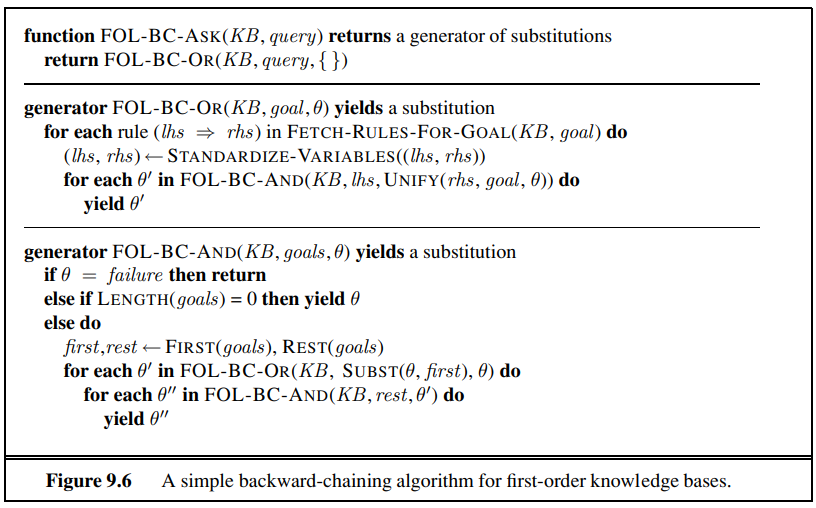
\includegraphics[]{images/backward-fol.png}
\end{center}
The figure above shows a backward-chaining algorithm for definite clauses. FOL-BC-ASK(KB,
goal) will be proved if the knowledge base contains a clause of the form $lhs \Rightarrow goal$, where $lhs$ (left-hand side) is a list of conjuncts. Backward chaining is a kind of AND/OR search, the OR part because the goal query can be proved by any rule in the knowledge base, and the AND part because all the conjuncts in the $lhs$ of a clause must be proved.  FOL-BC-OR works by fetching all clauses that might unify with the goal, standardizing the variables in the clause to be brand-new variables, and
then, if the $rhs$ of the clause does indeed unify with the goal, proving every conjunct in the $lhs$, using FOL-BC-AND. That function in turn works by proving each of the conjuncts in turn, keeping track of the accumulated substitution as we go.\\\\
Backward chaining, as we have written it, is clearly a depth-first search algorithm. This means that its space requirements are linear in the size of the proof. It also means that backward chaining (unlike forward chaining) suffers from problems with repeated states and \textbf{incompleteness}. This could be fixed by checking current goal against every goal on stack. This algorithm is widely used for \textbf{logic programming}.
\begin{center}
    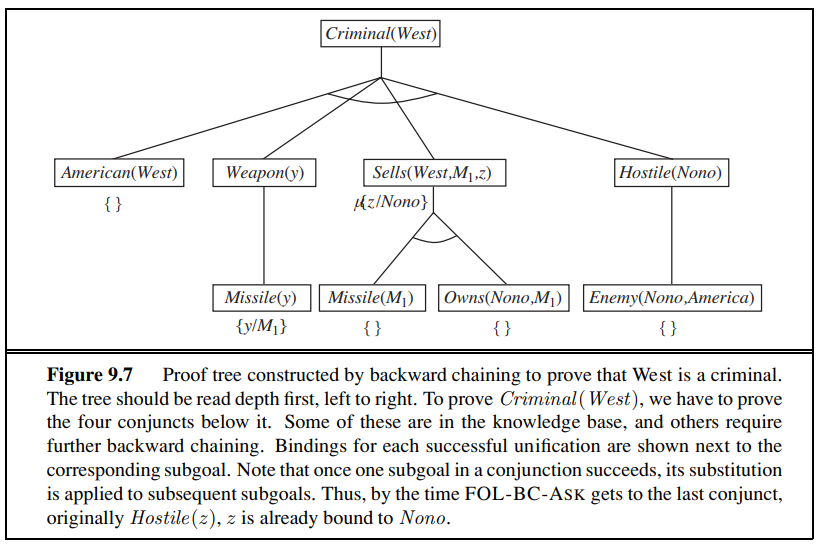
\includegraphics[]{images/backward-fol-tree.png}
\end{center}


\section{Logic programming}
Logic programming is a technology that comes fairly close to embodying the declarative ideal described before: that systems should be constructed by expressing knowledge in
a formal language and that problems should be solved by running inference processes on that knowledge.\\\\
\textbf{Prolog} is the most widely used logic programming language. Prolog programs are sets of definite clauses written in a notation somewhat different from standard first-order logic. Prolog uses uppercase letters for variables and lowercase for constants, the opposite of our convention for logic. Commas separate conjuncts in a clause,
and the clause is written “backwards” from what we are used to.  instead of $A \land B \Rightarrow C$ in Prolog we have $C :- A, B$.\\\\
The execution of Prolog programs is done through depth-first backward chaining, where clauses are tried in the order in which they are written in the knowledge base. There is a set of built-in functions for arithmetic. Literals using these function symbols are “proved” by executing code rather than doing further inference.
\\\\
The notation $[E|L]$ denotes a list whose first element is $E$ and whose rest is $L$. Here is a Prolog program for $append(X,Y,Z)$, which succeeds if list $Z$ is the result of appending lists $X$ and $Y$:
\begin{center}
    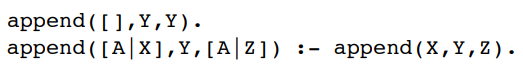
\includegraphics[]{images/prolog.png}
\end{center}
In English, we can read these clauses as (1) appending an empty list with a list $Y$ produces the same list $Y$ and (2) $[A|Z]$ is the result of appending $[A|X]$ onto $Y$, provided that $Z$ is the result of appending $X$ onto $Y$. We can ask the query $append(X,Y,[1,2])$: what two lists can be appended to give $[1,2]$? We get back the solutions:
\begin{center}
    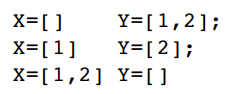
\includegraphics[]{images/prolog-sol.png}
\end{center}
